%%%%%%%%%%%%%%%%%%%%%%%%%%%%%%%%%%%%%%%%%
% Stylish Article
% LaTeX Template
% Version 2.1 (1/10/15)
%
% This template has been downloaded from:
% http://www.LaTeXTemplates.com
%
% Original author:
% Mathias Legrand (legrand.mathias@gmail.com) 
% With extensive modifications by:
% Vel (vel@latextemplates.com)
%
% License:
% CC BY-NC-SA 3.0 (http://creativecommons.org/licenses/by-nc-sa/3.0/)
%
%%%%%%%%%%%%%%%%%%%%%%%%%%%%%%%%%%%%%%%%%

%----------------------------------------------------------------------------------------
%	PACKAGES AND OTHER DOCUMENT CONFIGURATIONS
%----------------------------------------------------------------------------------------

\documentclass[10pt]{SelfArx} % Document font size and equations flushed left

\usepackage[english]{babel} % Specify a different language here - english by default

\usepackage{lipsum} % Required to insert dummy text. To be removed otherwise

\captionsetup[figure]{justification=justified, singlelinecheck=off} 
\captionsetup[table]{justification=justified, singlelinecheck=off} 

%----------------------------------------------------------------------------------------
%	COLUMNS
%----------------------------------------------------------------------------------------

\setlength{\columnsep}{0.55cm} % Distance between the two columns of text
\setlength{\fboxrule}{0.75pt} % Width of the border around the abstract
\linespread{1.5}

%----------------------------------------------------------------------------------------
%	COLORS
%----------------------------------------------------------------------------------------

\definecolor{color1}{RGB}{0,0,90} % Color of the article title and sections
\definecolor{color2}{RGB}{10,20,20} % Color of the boxes behind the abstract and headings
\definecolor{xsubj}{RGB}{243,194,68} 
\definecolor{xsess}{RGB}{53,99,161} 
\definecolor{xsamp}{RGB}{18,165,121} 

%----------------------------------------------------------------------------------------
%	HYPERLINKS
%----------------------------------------------------------------------------------------

\usepackage{hyperref} % Required for hyperlinks
\hypersetup{hidelinks,colorlinks,breaklinks=true,urlcolor=color2,citecolor=color1,linkcolor=color1,bookmarksopen=false,pdftitle={Title},pdfauthor={Author}}
%----------------------------------------------------------------------------------------
%	ARTICLE INFORMATION
%----------------------------------------------------------------------------------------

% \JournalInfo{Journal, Vol. XXI, No. 1, 1-5, 2013} % Journal information
\JournalInfo{$ $ } % Journal information
\Archive{Pre-print} % Additional notes (e.g. copyright, DOI, review/research article)

\PaperTitle{Data Augmentation Through Monte Carlo Arithmetic Leads to Improved Classifiers in Neuroimaging} % Article title

\Authors{Gregory Kiar\textsuperscript{1}, Yohan Chatelain\textsuperscript{2}, Ali Salari\textsuperscript{2}, Alan C. Evans\textsuperscript{1}, Tristan Glatard\textsuperscript{2}} % Authors
\affiliation{\textsuperscript{1}\textit{Montréal Neurological Institute, McGill University, Montréal, QC, Canada}}
\affiliation{\textsuperscript{2}\textit{Department of Computer Science and Software Engineering, Concordia University, Montréal, QC, Canada}}

\Keywords{Stability --- Network Neuroscience --- Neuroimaging --- Machine Learning --- Generalizability} % Keywords - if you don't want any simply remove all the text between the curly brackets
\newcommand{\keywordname}{Keywords} % Defines the keywords heading name

%----------------------------------------------------------------------------------------
%	ABSTRACT
%----------------------------------------------------------------------------------------

\Abstract{Machine learning models are commonly applied to human brain imaging datasets in an effort to associate
function or structure with behaviour, health, or other individual attributes. Such models often rely on low-dimensional
maps relating brain regions, generated by complex processing pipelines. However, the numerical instabilities inherent
to pipelines limits the fidelity of these estimates, and results in bias-rich derivatives serving as inputs to machine
learning models. This work seeks to take advantage of numerical instabilities in pipelines by inducing numerical
perturbations, ultimately producing a range of results and reducing the bias in networks. We found that resampling
brain networks across a series of numerically perturbed outcomes led to improved performance in all tested classifiers,
preprocessing strategies, and dimensionality reduction techniques when tasked with an age classification task.
Importantly, we find that this benefit does not hinge on a large number of perturbations, suggesting that even
minimally perturbing a dataset adds meaningful variance which can be captured in the subsequently designed models.}

%----------------------------------------------------------------------------------------

\begin{document}

\flushbottom % Makes all text pages the same height
\maketitle % Print the title and abstract box
% \tableofcontents % Print the contents section
\thispagestyle{empty} % Removes page numbering from the first page

%----------------------------------------------------------------------------------------
%	ARTICLE CONTENTS
%----------------------------------------------------------------------------------------
\pagestyle{fancy}
\section*{Introduction}

The application of machine learning has become commonplace for the identification and characterization of individual
biomarkers in neuroimaging~\cite{woo2017building}. Models may be applied to discriminate between measures of brain
structure or function based upon phenotypic variables related to
disease~\cite{Crossley2014-tg,Payabvash2019-tm,Tolan2018-nq}, development~\cite{Zhang2019-ko}, or other axes of
potential consequence~\cite{Zhu2018-cs,Park2015-uj}.

These models often build representations upon processed imaging data, in which 3D or 4D images have been transformed
into estimate of structure~\cite{wade2017machine}, function~\cite{weis2020sex}, or
connectivity~\cite{munsell2015evaluation}. However, there is a lack of reliability in these estimates, including
variation across analysis team~\cite{botvinik2020variability}, software library~\cite{bowring2019exploring}, operating
system~\cite{salari2020file}, and instability in the face of numerical noise~\cite{Kiar2020-kz}. This uncertainty
limits the ability of models to learn generalizable relationships among data, and leads to bias-rich predictors.
Traditionally, this bias has been reduced through the collection and application of repeated-measurement
datasets~\cite{sudlow2015uk,zuo2014open}, though this requires considerable resources and is not feasible in the
context of all clinical populations.

Perturbation methods which inject small amounts of noise throught the execution of a pipeline, such as Monte Carlo
Arithmetic (MCA)~\cite{Parker1997-qq,Denis2016-wo}, have recently been used to induce instabilities in structural
connectome estimation software~\cite{Kiar2020-lb}. Importantly, this technique produces a range of equally plausible
results, where no single observation is more or less valid than the others – including those which were left
unperturbed. While the impact that sampling from a set of perturbed connectomes may have on learning brain-phenotype
relationships~\cite{Kiar2020-kz}, there remains potential for leveraging the distribution of results to augment
datasets in lieu of increasing sample sizes or performing repeated measurements.

Using an existing collection of MCA-perturbed structural connectomes~\cite{Kiar2020-yz}, we trained classifiers on
networks sampled from the distribution of results and evaluated their performance relative to using only the
unperturbed networks. We evaluate several techniques for resampling the networks, and compare classifiers through their
validation performance, the performance on an out-of-sample test set, and the generalizability of their performance
across the two. We demonstrate the efficacy of using MCA as a method for dataset augmentation which leads to more
robust and generalizable models of brain-phenotype relationships.


\section*{Materials \& Methods}

The objective of this study was to evaluate the impact of aggregating collections of unstable brain networks towards
learning robust brain-phenotype relationships. We sampled and aggregated simulated networks within individuals to learn
relationships between brain connectivity and individual an trait, in this case age, and compared this to traditional
baseline performance on this tasks. We compared aggregation strategies with respect to baseline validation performance,
performance out-of-sample, and generalizability.

All developed software and analysis resources for this project have been made available through GitHub at
\url{https://github.com/gkpapers/2020AggregateMCA}.

\subsection*{Dataset}

An existing dataset containing Monte Carlo Arithmetic (MCA) perturbed structural human brain networks was used for
these experiments~\cite{Kiar2020-yz}. The perturbations introduced for the generation of brain networks in this dataset
were at the level of machine-error, simulating expected error over a typical pipeline execution. This dataset contains
a single session of data from $100$ individuals ($100\times 1 \times1$). The derived brain networks were generated with
a probabilistic structural connectome estimation pipeline~\cite{Garyfallidis2014-ql} using a fixed random seed, and
Monte Carlo Arithmetic (MCA) perturbations were added to all Python-implemented operations throughout the
pipeline~\cite{Denis2016-wo,Parker1997-qq}. Each sample was simulated $20$ times, resulting in $2,000$ unique graphs.
Further information on the processing and curation of this dataset can be found here~\cite{Kiar2020-kz}.

This collection enabled the exploration of subsampling and aggregation methods in a typical learning context for
neuroimaging~\cite{Dimitriadis2017-pd,Buchanan2014-pm}. Exploring the relationship between the number of simulations
and performance further allows for MCA-enabled resampling to be evaluated as a method of dataset augmentation.

As the target for classification, individual-level phenotypic data strongly implicated in brain connectivity was
desired. Participant age, which has consistently been shown to have a considerable impact on brain
connectivity~\cite{Meier2012-ve,Wu2012-uc,Bookheimer2019-ti,Zhao2015-rm}, was selected and turned into a binary target
by dividing participants into adult ($>18$) and non-adult groups ($68\%$ adult).

\subsection*{Preprocessing}
Prior to being used for this task, the brain networks being were represented as symmetric $83 \times 83$ adjacency
matrices, sampled upon the Desikan-Killiany-Tourville~\cite{Klein2012-vi} anatomical parcellation. To reduce redundancy
in the data, all edges belonging to the upper-triangle of these matrices were preserved and vectorized, resulting in a
feature vector of $3,486$ edges per sample. All samples were preprocessed using one of four standard techniques:

\paragraph{Raw} The raw streamline count edge-weight intensities were used as originally calculated.

\paragraph{Log Transform} The log10 of edge weights were taken, and edges with $0$ weight prior to the transform were
reset to $0$.

\paragraph{Rank Transform} The edges were ranked based on their intensity, with the largest edge having the maximum
value. Ties were settled by averaging the rank, and all ranks were finally min-max scaled between $0$ and $1$.

\paragraph{Z-Score} The edge weights were z-scored to have a mean intensity of $0$ and unit variance.

\subsection*{Machine Learning Pipelines}

The preprocessed connectomes were fed into pipelines consisting of two steps: dimensionality reduction and
classification. Dimensionality reduction was applied using one of two methods:

\paragraph{Principal Component Analysis} The connectomes were projected into the $20$ dimensions of highest variance.
The number of components was chosen to capture approximately $90\%$ of the variance present within the dataset.

\paragraph{Feature Agglomeration} The number of features in each connectome were reduced by combining edges according
to maximum similarity/minimum variance using agglomerative clustering~\cite{Ward1963-uh}. The number of resulting
features was $20$, to be consistent with the number of dimensions present after PCA, above.

After dimensionality reduction, samples were fed into one of five distinct classifiers as implemented through scikit
learn~\cite{Pedregosa2011-uz}:

\paragraph{Support Vector Machine} The model was fit using a radial basis function (RBF) kernel, L2 penalty, and a
balanced regularization parameter to account for uneven class membership.

\paragraph{Logistic Regression} A linear solver was used due to the relatively small dataset size. L2 regularization
and balanced class weights were used, as above.

\paragraph{K-Nearest Neighbour} Class membership was determined using an L2 distance and the nearest $10\%$ of
samples, scaling with the number of samples used for training.

\paragraph{Random Forest} $100$ decision trees were fit using balanced class weights, each splitting the dataset
according to a maximum of $4$ features per node (corresponding to the rounded square root of $20$ total features).

\paragraph{AdaBoost} A maximum of $50$ decision trees were fit sequentially such that sample weights were iteratively
adjusted to prioritize performance on previously incorrectly-classified samples, consistent with~\cite{Freund1997-qy}.

The hyperparameters for all models were refined from their default values to be appropriate for a small and imbalanced
dataset. The performance for all pipeline combinations of preprocessing methods, dimensionality reduction techniques,
and models using the reference (i.e. unperturbed) executions in the dataset ranged from an F1 score of $0.64 – 0.875$
with a mean of $0.806$; this evaluation was performed on a consistent held-out test set which was used for all
experiments, as described in a following section. This set of models was chosen as it includes i) well understood
standard techniques, ii) both parametric and non-parametric methods, iii) both ensemble and non-ensemble
methods, and iv) models which have been commonly deployed for the classification neuroimaging
datasets~\cite{Meier2012-ve,Tunc2016-cz, Zhu2018-cs,Payabvash2019-tm,Crossley2014-tg,Park2015-uj,Nayak2016-wl,Tolan2018-nq}.

\subsection*{Dataset Sampling}

A chief purpose of this manuscript involves the comparison of various forms of aggregation across
equivalently-simulated pipeline outputs. Accordingly, the dataset was resampled prior to dimensionality reduction and
classifiers were trained, evaluated, and combined according to the following procedures:

\paragraph{Reference} Networks generated without any MCA perturbations were selected for input to the models, serving
as a benchmark.

\paragraph{Truncate} The number of significant digits~\cite{Parker1997-qq} per-edge was calculated using all
simulated networks, and the edge weights in the reference graph were truncated to the specified number of digits.
Importantly, this is the only method used which deliberately squashes the variance observed across simulations.

\paragraph{Jackknife} The datasets were repeatedly sampled such that a single randomly chosen observation of each
unique network was selected (i.e. derived from the same input datum). This resampling was performed $100$ times,
resulting in the total number of resamplings being $5\times$ larger than the number of unique observations per network,
ensuring a broad and overlapping sampling of the datasets.

\paragraph{Median} The edgewise median of all observations of the same network were used as the samples for training
and evaluation.

\paragraph{Mean} Similar to the above, the edgewise mean of all observations for each network were computed and used
as input data to the classifiers in both collections.

\paragraph{Consensus} A distance-dependent average network~\cite{Betzel2018-eo} was computed across all observations
of each network. This data-aware aggregation method, developed for structural brain network analysis, preserves network
properties often distorted when computing mean or median networks.

\paragraph{Mega-analysis} All observations of each network were used simultaneously for classification, increaseing
the effective sample size. Samples were organized such that all observations of the same network only appeared within a
single fold for training and evaluation, ensuring double-dipping was avoided.

\paragraph{Meta-analysis} Individual classifiers trained across jackknife dataset resamplings, above, were treated as
independent models and aggregated into an ensemble classifier. The ensemble was fit using a logistic regression
classifier across the outputs of the jackknifed classifiers to learn a relationship between the predicted and true
class labels.

The robustness and possible benefit of each subsampling approach was measured by evaluation on a subset of all MCA
simulations, including $9$ distinct numbers of simulations, ranging from $2$ to $20$ simulations per sample. Combining
the dataset sampling methods, the set of simulations, preprocessing strategies, dimensionality reduction techniques,
and classifier models, there were $2,560$ models trained and evaluated.

\subsection*{Training \& Evaluation}

Prior to training models on the brain networks, $20\%$ of subjects were excluded from each dataset for use as an
out-of-sample test dataset for all experiments. With the remaining $80\%$ of subjects, cross validation was performed
following a stratified grouped $k$-fold approach ($k=5$). In this approach, samples were divided into training and
validation sets such that the target variable was proportionally represented on each side of the fold (stratified),
conditional upon all observations from the same individual, relevant for the mega-analysis dataset sampling method,
falling upon the same side of the fold (grouped). This resulted in $5$ fold-trained classifiers per configuration, each
trained on $64\%$ of the samples and validated on $16\%$, prior to each being tested on the remaining $20\%$ of
held-out samples. All random processes used in determining the splits used the same seed to remove the effect of random
sampling.

Classifiers were primarily evaluated on both the validation and test (out-of-sample) sets using F1 score, a standard
measure for evaluating classification performance. The generalizability of predictions was defined as:

\begin{equation}
G = 1 - \lvert F1_{test} - F1_{validation} \rvert
\label{eq:gen}
\end{equation}

\begin{figure*}[bth!]\centering
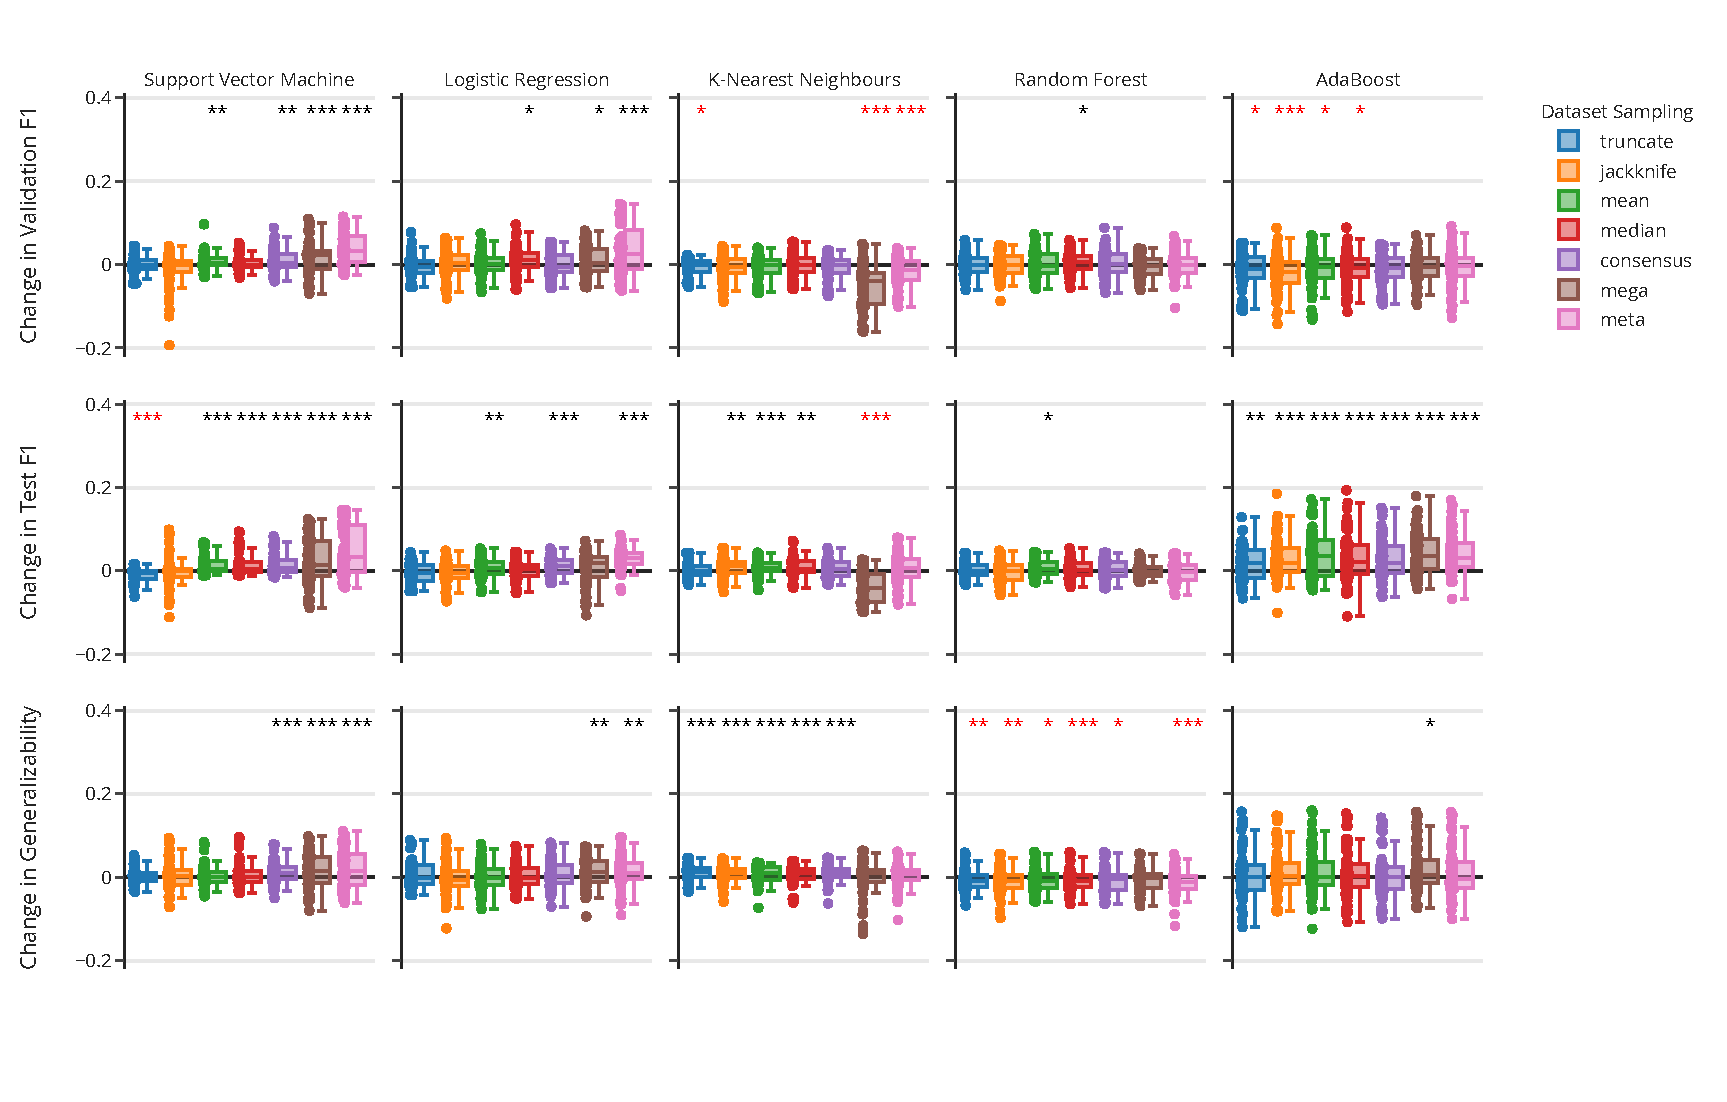
\includegraphics[width=\linewidth]{figures/1.pdf}
\caption{Relative change in classifier performance with respect to classifier type and dataset sampling strategies as
measured by change in F1 score on the validation set (top) or test set (middle), as well as the generalizability of
performance (bottom). Each star annotation indicates an order of magnitude of statistically significant change,
beginning at $0.05$ for one star and decreasing from there, with those in black or red indicating an increase or
decrease due to resampling, respectively.}
\label{fig:overall_perf}
\end{figure*}

where a score of $1$ (maximum) indicates the equivalent performance across both the validation and test sets, and a
lower score (minimum of $0$) indicates inconsistent performance. The absolute change in performance was used in
Eq.~\ref{eq:gen}, resulting in a score which penalizes spurious over-performance similarly to under-performance. This
is a desired attribute of the measure as all inconsistency, whether due to ``luck'' or model fit, is undesirable when
applying a classifier out-of-sample.

Differences in F1 score and generalizability for perturbed experiments with respect to their reference were used to
measure the change in performance between for each dataset sampling technique, and statistical comparisons were made
through Wilcoxon Signed-Rank tests.


%------------------------------------------------
\section*{Results}

The figures and findings presented in this section represent a summary of the complete experiment table which consists
of performance measures and metadata for all $2,200$ models tested. The complete performance table alongside the table
of significant differences, are made available through the GitHub repository.

\subsection*{Data Resampling Improves Classification}

\begin{table}[tbh]
\centering
\caption{Statistically significant change in performance from reference models. Red values indicate significant
decline in performance, empty cells indicate no significant change, and black values indicate significant improvement.
A single star representes $p < 0.05$, and each additional star is an additional order of magnitude of significance.}
\label{tab1:perf}
\small
\begin{tabular}{rccc}
\textbf{Dataset Sampling}  & \textbf{Validation} &      \textbf{Test} & \textbf{Generalizability} \\
\midrule
\textbf{Truncate}          &    {\color{red} **} &                    &                           \\
\textbf{Jackknife}         &    {\color{red} **} &                 ** &                           \\
\textbf{Mean}              &                     &                *** &                           \\
\textbf{Median}            &                     &                *** &                           \\
\textbf{Consensus}         &                     &                *** &                         * \\
\textbf{Mega-Analysis}     &     {\color{red} *} &                  * &                       *** \\
\textbf{Meta-Analysis}     &                  ** &                *** &                         * \\
\end{tabular}

\end{table}

The change in performance for each model and dataset sampling technique is shown in Figure~\ref{fig:overall_perf}. The
change in performance was measured as a change in F1 score on the validation set, the change in F1 score on the test
set, and the change in overall generalizability, a measure which summarizes the similarity between validation and test
performance for a given model. The overall performance of each subsampling method across the sets is summarized in
Table~\ref{tab1:perf}.

The support vector machine and logistic regression models improve across each of these three measures for a variety of
dataset sampling techniques, suggesting that the addition of the MCA-perturbed samples improves the training, testing,
and overall generalizability of the classifiers.

Distinctly, k-nearest neighbours (KNN) and AdaBoost classifiers experienced minimal change in validation and often saw
their perfomance decline. However, the improvement of these classifiers on the test set suggests that resampling
reduced overfitting in these classifiers. In the case of KNN, this translates to imrpoved generalizability, while in
the case of AdaBoost generalizability was largely unchanged, suggesting that the model went from underperforming to
overperforming after dataset resampling. The unique decline in performance when using the mega-analytic resampling
technique on KNN classifier is suggestive of poor hyperparameterization, as there is a strong relationship between the
number of samples in the dataset and the $k$ parameter of the model. At present this parameter was scaled linearly with
the number of MCA simulations used, however, it is both possible that an improved scaling function exists or that the
model performance degrades with large sample sizes making it a poor model choice given this resampling technique.

The random forest classifiers uniquely did not see a significant change in validation or testing performance across the
majority of resampling techniques. However, these classifiers did experience a significant decrease in the
generalizability of their performance, meaning that there was a larger discrepancy between training and testing
performance in many cases. This distinction from the other models is likely due to the fact that random forest is a
simple ensemble technique which takes advantage of training many independent classifiers and samples them to assign
final class predictions. It is likely that this approach forms more generalizable predictions generally, and thus the
addition of more data does not significantly improve performance further. While AdaBoost is also an ensemble method,
the iterative training of models with increasing emphasis on difficult samples allows for the added variance in those
samples to play an increasingly central role in the construction of class relationships.

\begin{figure*}[bht!]\centering
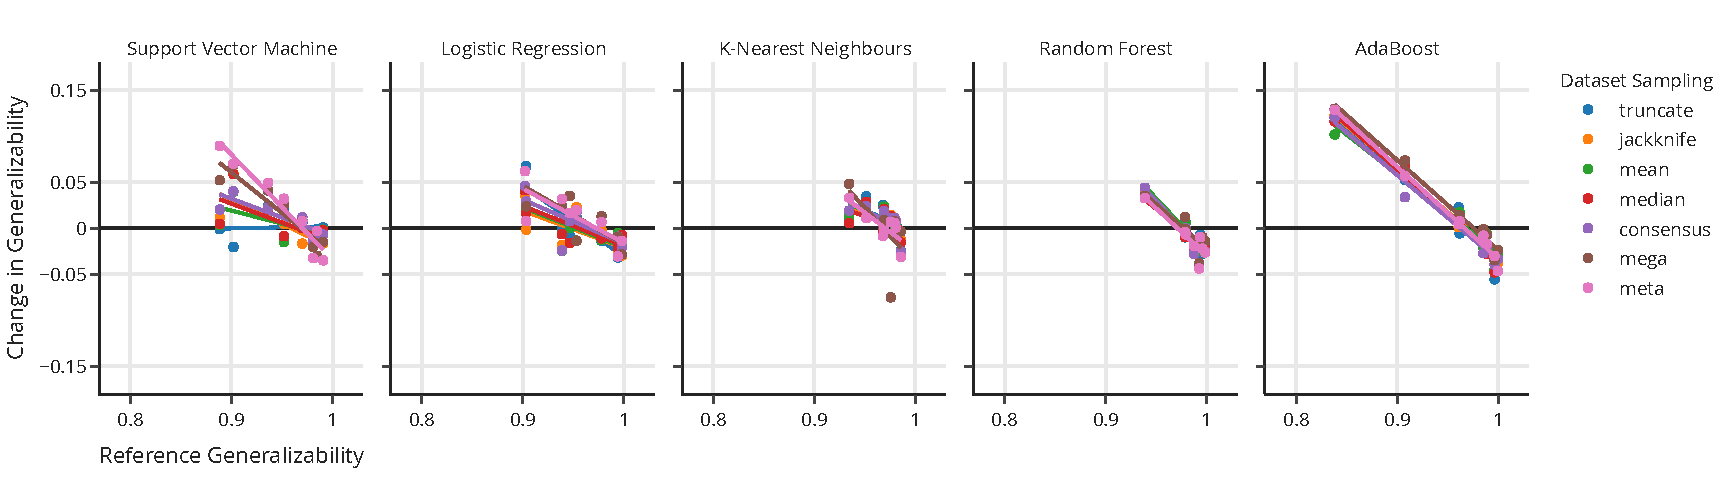
\includegraphics[width=\linewidth]{figures/2a.pdf}
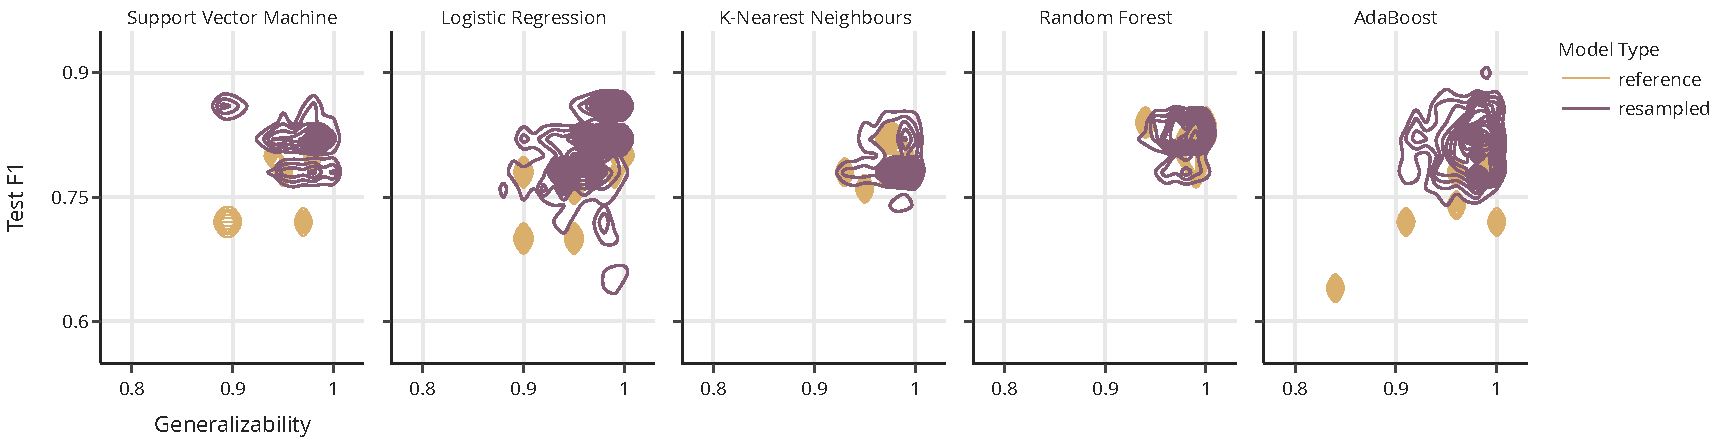
\includegraphics[width=\linewidth]{figures/2b.pdf}
\caption{Relationship between generalizability and resampling. Top: change in the generalizability of classifiers with
respect to the reference generalizability. Each data point represents the mean change in generalizability for all
models using the same preprocessing and dimensionality reduction techniques for a given classifier and dataset sampling
strategy. Bottom: contour density distributions of generalizability and F1 scores across all models for both reference
and resampled training.
% The vertical lines for each plot represent the mean generalizability for the associated models.
}
\label{fig:change_in_gen}
\end{figure*}

\begin{figure*}[ht]\centering
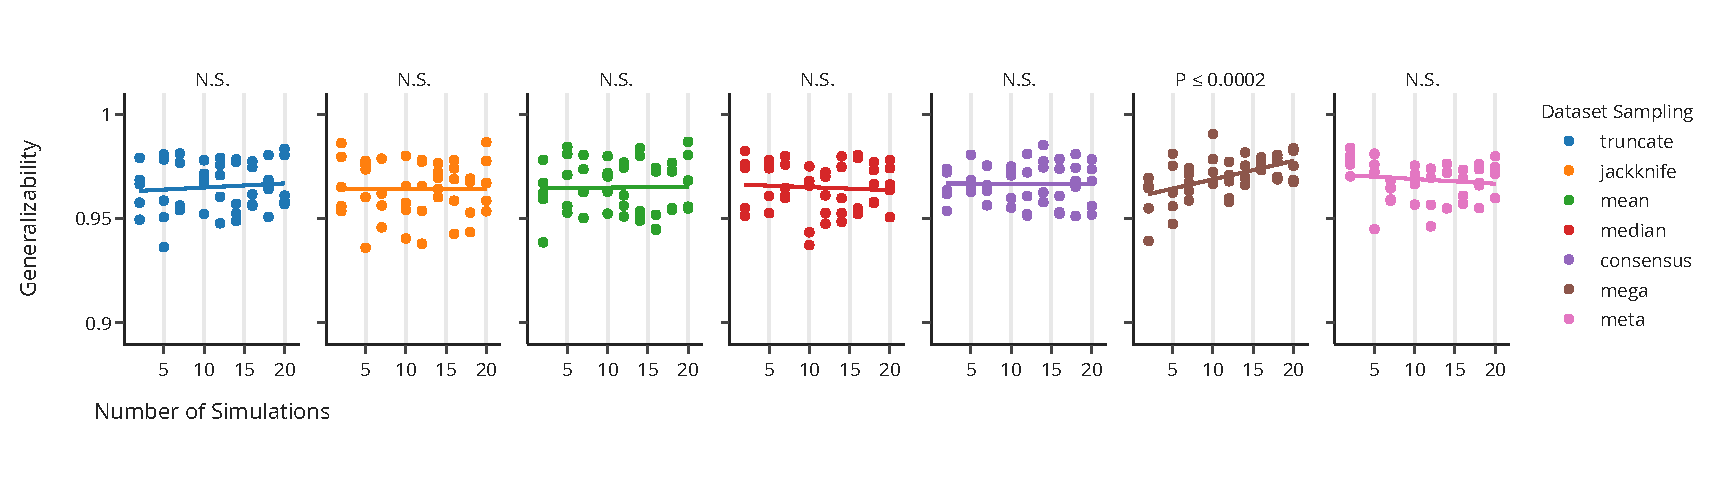
\includegraphics[width=\linewidth]{figures/3.pdf}
\caption{The generalizability of classifiers using each dataset sampling technique with respect to the number of MCA
simulations. Each number of simulations was sampled a single time, to avoid artificial skewing of the dataset due to
the inclusion of ``higher'' or ``lower'' quality samples; a single drawing of each split mimics a true perturbation
experiment context.}
\label{fig:nmca}
\end{figure*}


Across all classifier types, it was found that consensus, mega-, and meta-analytic approaches outperformed other
dataset resampling methods in that each led to improved testing performance and generalizability. The only method which
did not improve performance at all was the truncation resampling. This method was distinct from the others in that the
variance observed across simulations was used to squash variance in the reference network, whether other approaches
captured the variance. The finding that truncation hurts performance importantly suggests that the variability across
the observed network is biologically meaningful and contains signal.

While certain combinations of preprocessing, dimensionality reduction, and classifiers performed more harmoniously than
others, there was no significant relationship between the performance of any single resampling method and preprocessing
or dimensionality reduction technique. The above results show that dataset augmentation through MCA-perturbed pipeline
outputs may be an effective way to improve the performance and generalizability of non-ensemble classifiers tasked with
modeling brain-phenotype relationships, both within and out of sample, especially when variance is captured rather than
removed.

\subsection*{Resampling Leads to Consistent Performance}

To beter characterize the the benefit of resampling, the relationship between the magnitude of improvement and the
baseline performance of the classifer were further explored (Figure~\ref{fig:change_in_gen}). We found that the
increase in the generalizability of a classifier was inversely related to the baseline generalizability
(Figure~\ref{fig:change_in_gen}; top). In other words, the less generalizable a classifier was originally, the more its
generalizability improved (significant at $p < 0.05$ for all dataset sampling strategies and classifier other than
KNN). There were several situations in which the generalizability of models were noted to decrease, however, though
this only occurred for models with high generalizability scores (all $>0.935$). Importantly, the relative change in
generalizability shifts scores towards a single ``mode'', suggesting a less biased estimate of the true
generalizability of performance on the task, and mitigating both under- and over-performance due to chance.

When exploring the relationship between F1 and generalizability (Figure~\ref{fig:change_in_gen}; bottom), it becomes
apparent that even for the majority of models which may not have improved performance along both axes, either their
generalizability or F1 score is improved. While an ideal classifier would reside in the top-right of the shown plots,
the dataset resampling techniques consistently shift the distributions in this direction and improve classifiers along
one if not both of these axes. Importantly, the variance in performance across both of these axes is significantly
decreased, suggesting that resampling lead to the development of more reliable and reproducible classifiers.

\subsection*{Number of Simulations is Largely Unimpactful}

While we previously note an increase in classifier performance due to perturbation-enabled dataset resampling, it was
important to explore the relationship between the number of simulated samples and the performance
(Figure~\ref{fig:nmca}). There was no relationship between the number of independent simulations and performance, as
measured by either F1 or generalizability, for all dataset resampling techniques other than mega-analysis. In the case
of the mega-analytic approach, however, there was a significant positive relationship between the number of samples
used and the generalizability of performance, though there remained no increase in F1 score. The mega-analysis approach
is the only approach which changes the number of samples being provided directly to the classifiers, thus mimics an
increase in sample size for traditional experiments. While outlying samples may play a small role in many of the
proposed forms of resampling, or non-existent in the median case, the mega analytic approach treats all simulations
with equal importance as unique samples in the dataset. It is for this reason that the observed relationship here
is consistent to what one would expect when increasing the number of samples in their experiment.

\section*{Discussion}

The numerical perturbation of analytic pipelines provides a unique, data-agnostic, and computationally unintrusive
method for dataset augmentation. Using a technique such as MCA, samples can be simulated across an array of controlled
executions and used to enrich datasets across a range of plausible results. We demonstrate that this method of dataset
augmentation can be used to improve the training, testing, and generalizability of classifiers.

Through the training and evauation of $2,560$ models combining varying strategies for preprocessing, dimensionality
reduction, classifier, and resampling, we found consistent improvement across all measured axes. Interestingly, while
there was a statistically significant improvement when using many dataset resampling techniques, there was no
significant improvement, and in fact a reduction, in the performance of the truncation method. This result importantly
demonstrates that the added variability in results obtained through MCA is meaningful and signal-rich itself, and the
most important determination of performance is the inclusion of this variability.

While the non-ensemble methods benefited most obviously from the dataset resampling strategies, where both F1 and
generalizability were often improved, the results presented in Figure~\ref{fig:change_in_gen} demonstrate that
variability in performance across both of these axes was reduced across all classifier configurations. While a
reduction in variability of performance is desirable in itself, this figure also illustrates that the performance of
resulting models converges around the more performant models in the case of all classifers.

Although performance was improved by the integration of MCA simulated samples, performance was not significantly
related to the number of simulations used in any case other than the mega-analytic resampling strategy. The
independence of performance and number of simulations is encouraging, as a key limitation for using Monte Carlo methods
is the often extreme computational overhead. The ability to use a small number of simulations and achieve equivalent
performance through the majority of resampling techniques allows for significantly better performance without either
added data collection and a theoretical doubling the sample processing time. The benefit of increasing the number of
simulations in the mega-analytic case could be considered an analog to increasing the sample size of an experiment.
While the range of simulations used here demonstrated a consistent improvement in generalizability, there will be a
plateau in performance, either at the maximum achievable score or, more likely, before this is reached. Further
work is required for characterizing the relationship between the performance of mega-analytic resampling and the number
of simulations, and it is likely that this relationship will be domain-specific.

An important limitation of our claim that classifiers with poorer baseline performance benefit more from augmentation
is the limit to which that claim remains true. For example, it is unlikely that the trend observed here, with a mean
baseline performance of $0.81$, would hold across models operating with baseline performance near chance.
Characterizing the behaviour of this technique across a range of classification contexts and performances would shed
light on whether this technique could be applied globally or if it is limited to making ``good'' models better.

It is a well understood problem that small sample sizes lead to uncertainty in modeling~\cite{varoquaux2018cross}.
This is generally planned for in one of two ways: the collection of vast datasets, as is the case in the UK-BioBank
which strives to collect samples from half a million individuals~\cite{sudlow2015uk}), or the collection of repeated
measurements from the selected samples, as is the case in the Consortium of Reliability and Reproducibility which
orchestrates multiple centres and scanners, each collecting multiple acquisitions~\cite{zuo2014open}. In either case,
the additional data collection by these initiatives is both financially and temporally expensive and leads to
unintended confounding effects associated with time of day~\cite{vandewalle2009functional},
weather~\cite{di2019estimations}, or other off-target variables that are poorly described in the resulting
dataset~\cite{chaddock2010neuroimaging}. While the results presented here provide strong evidence in favour of dataset
augmentation through numerical perturbations, the improvement from these methods has not be situated relative to
additional data acquisition due to the limited sample size of the available perturbed repeated-measures
dataset~\cite{Kiar2020-yz}. While it is likely that the methods demonstrated here will work harmoniously with
traditional methods of dataset augmentation, it is presently unclear if this technique could serve as a cost-effective
replacement for data collection, and exploring that relationship is an exciting avenue for future work.

A common issue in many machine learning contexts is the unbalanced nature of datasets. When using a nearest-neighbour
classifier, for instance, a dramatic difference the membership of each group could have significant impact on model
hyper-parameters and performance. In contexts where improved sampling is not possible, such as when considering a
clinical population, perturbation-augmented datasets could be applied for realistic upsampling of data. In this case, a
mega-analytic aggregation strategy could be used in which more simulations would be performed for members of the
under-represented class, similar to the balancing of weights applicable to some models. This application is
particularly important, as upsampling is often challenging in biological contexts where realistic simulation models are
sparse.


\section*{Conclusion}

This work demonstrates the benefit of augmenting datasets through numerical perturbations. We present an approach which
leverages the numerical instability inherent to pipelines for creating more accurate and generalizable classifiers and
representations of brain-phenotype relationships. While the approach and results demonstrated here were specifically
relevant in the context of brain imaging, the data-agnostic method for inducing perturbations and off-the-shelf machine
learning techniques used suggest that this approach may be widely applicable across domains. This work uniquely shows
that numerical uncertainty is an asset which can be harnessed to increase the signal captured from datasets and
lead to more robust learned relationships.


\subsection*{Data \& Code Availability}
The perturbed connectomes were publicly available data resource previously produced and made available by the
authors~\cite{Kiar2020-yz}. They can be found persistently at \url{https://doi.org/10.5281/zenodo.4041549}, and are
made available through The Canadian Open Neuroscience Platform (\url{https://portal.conp.ca/search}, search term
"Kiar"). All software developed for processing or evaluation is publicly available on GitHub at
\url{https://github.com/gkpapers/2020AggregateMCA}. Experiments were launched on Compute Canada's HPC cluster
environment. 

\subsection*{Author Contributions}
GK was responsible for the experimental design, data processing, analysis, interpretation, and the majority of writing.
All authors contributed to the revision of the manuscript. TG and ACE contributed to experimental design, analysis,
interpretation. The authors declare no competing interests for this work. Correspondence and requests for materials
should be addressed to Gregory Kiar at \url{gregory.kiar@mail.mcgill.ca}.

\subsection*{Acknowledgments} 
This research was financially supported by the Natural Sciences and Engineering Research Council of Canada (NSERC)
(award no. CGSD3-519497-2018). This work was also supported in part by funding provided by Brain Canada, in partnership
with Health Canada, for the Canadian Open Neuroscience Platform initiative.

%----------------------------------------------------------------------------------------
%	REFERENCE LIST
%----------------------------------------------------------------------------------------
% \phantomsection
\bibliographystyle{IEEEtran}
\bibliography{aggregating-unstable-derivatives}


\end{document}
